\section{Performance test}
This section contains the results from the performance test done by the subjects. First of the results from the regressor trained only with EMG data are presented, and afterwards compared to the regressor trained with inclusion of IMU data. The boxplot in \ref{fig:GotItTime} shows the test scores of all limb positions for both features.

\begin{figure}[H]
	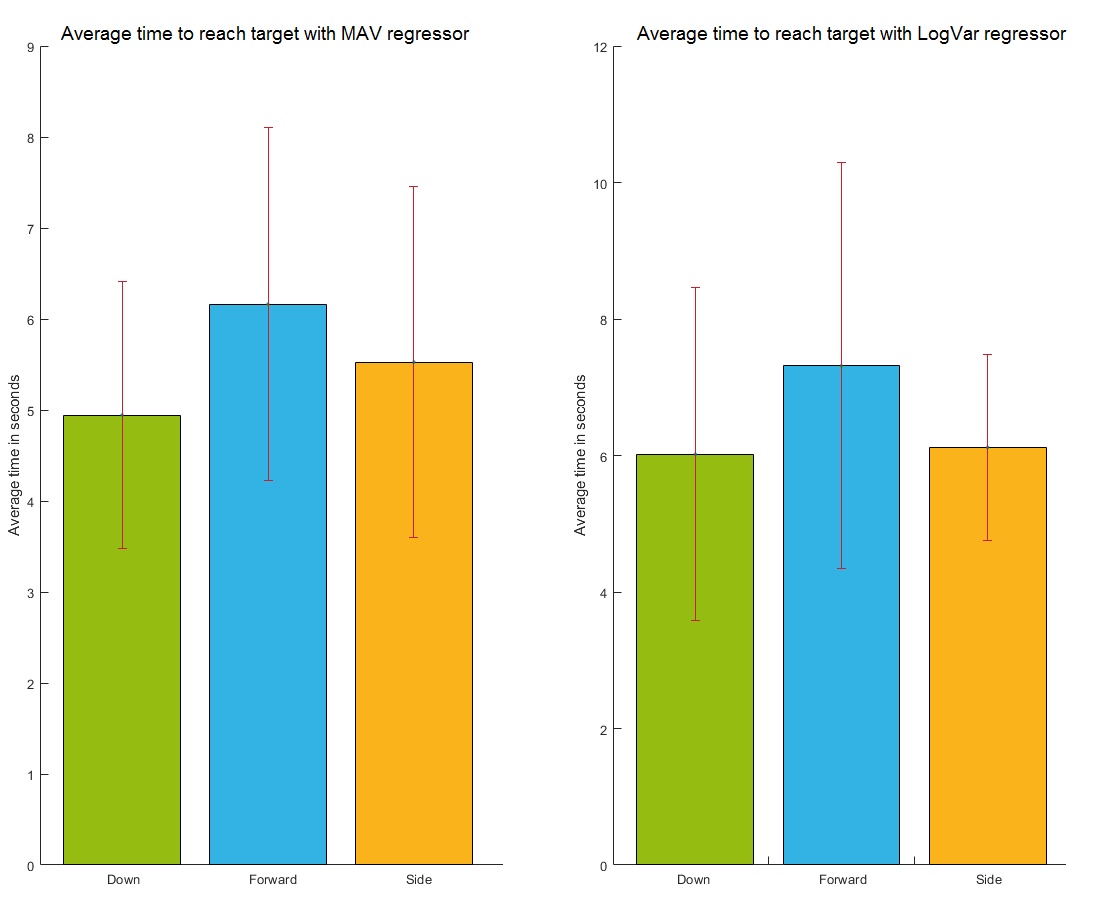
\includegraphics[width=0.7\textwidth]{figures/results/GotItTime}  %<--but is not needed.
	\caption{Calculated performance scores of the regressors. The bar chart illustrates the mean score across all subjects in the different limb positions, and the error bar illustrates the standard deviation}
	\label{fig:GotItTime}  %<--give the figure a label, so you can reference!
\end{figure}

	\begin{center}
		\begin{tabular}{l l l}
			\toprule
			\textbf{Limb position and feature} & \textbf{Overall mean error} & \textbf{Standard deviation}\\
			\midrule
			Down, MAV & 5.3377 & $\pm 1.5696$ \\
			Forward, MAV & 8.1791 & $\pm 4.7145$ \\
			Side, MAV & 6.0490 & $\pm 2.0490$ \\
			Down, LogVar & 6.5404 & $\pm 2.5315$ \\
			Forward, LogVar & 7.9123 & $\pm 3.4572$ \\
			Side, LogVar & 6.9325 & $\pm 2.3036$ \\
			\bottomrule
		\end{tabular}
		\captionof{table}{Test scores for the different limb for MAV and LogVar regressors}
	\end{center}

A one-sample Kolmogorov-Smirnov test was done on the scores from the MAV and LogVar respectively and showed no normality in both score sets(p = $7 * 10^{-20}$, $8 * 10^{-20}$ ). A Friedman's test was therefore applied for statistical analysis. The performance scores between the three limb positions prove not to be significantly different (p = 0.57), when applying the LogVar trained regressors in the online test. For the MAV trained regressors the performance score between all limb positions can not be proven significantly different either(p = 0.16). When comparing all performance scores from the two feature trained regression control schemes, the Friedman's test proves no significant difference (LogVar: 6.5 s, MAC: 5.5 s; p = 0.13).

\begin{figure}[H]
	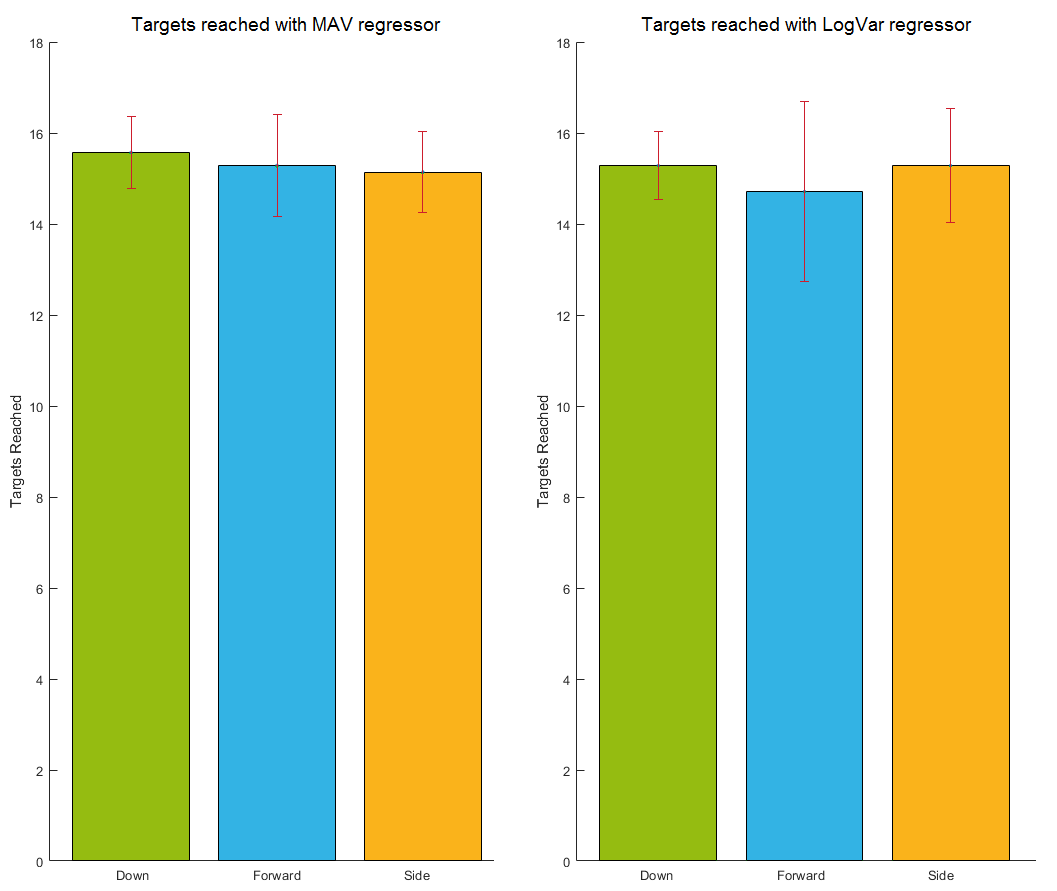
\includegraphics[width=0.7\textwidth]{figures/results/TargetsReached}  %<--but is not needed.
	\caption{The boxplot illustrates the amount of targets reached for the respective limb positions for both features.}
	\label{fig:TargetsReached}  %<--give the figure a label, so you can reference!
\end{figure}

	\begin{center}
		\begin{tabular}{l l l}
			\toprule
			\textbf{Limb position and feature} & \textbf{Overall mean error} & \textbf{Standard deviation}\\
			\midrule
			Down, MAV & 15.5556 & $\pm 0.7265$ \\
			Forward, MAV & 15.1111 & $\pm 1.0541$ \\
			Side, MAV & 15.2222 & $\pm 0.8333$ \\
			Down, LogVar & 15.4444 & $\pm 0.7265$ \\
			Forward, LogVar & 15 & $\pm 1.8020$ \\
			Side, LogVar & 15.3333 & $\pm 1.1180$ \\
			\bottomrule
		\end{tabular}
		\captionof{table}{Targets reached in the target test with the MAV and LogVar regressors.}
	\end{center}

A qualitative examination of the box plot in \ref{fig:TargetsReached} shows no significant difference in targets reached between limb positions and between all limb positions for the two features, which is similar to the Friedman's test results for the time per reached target.

\begin{figure}[H]
	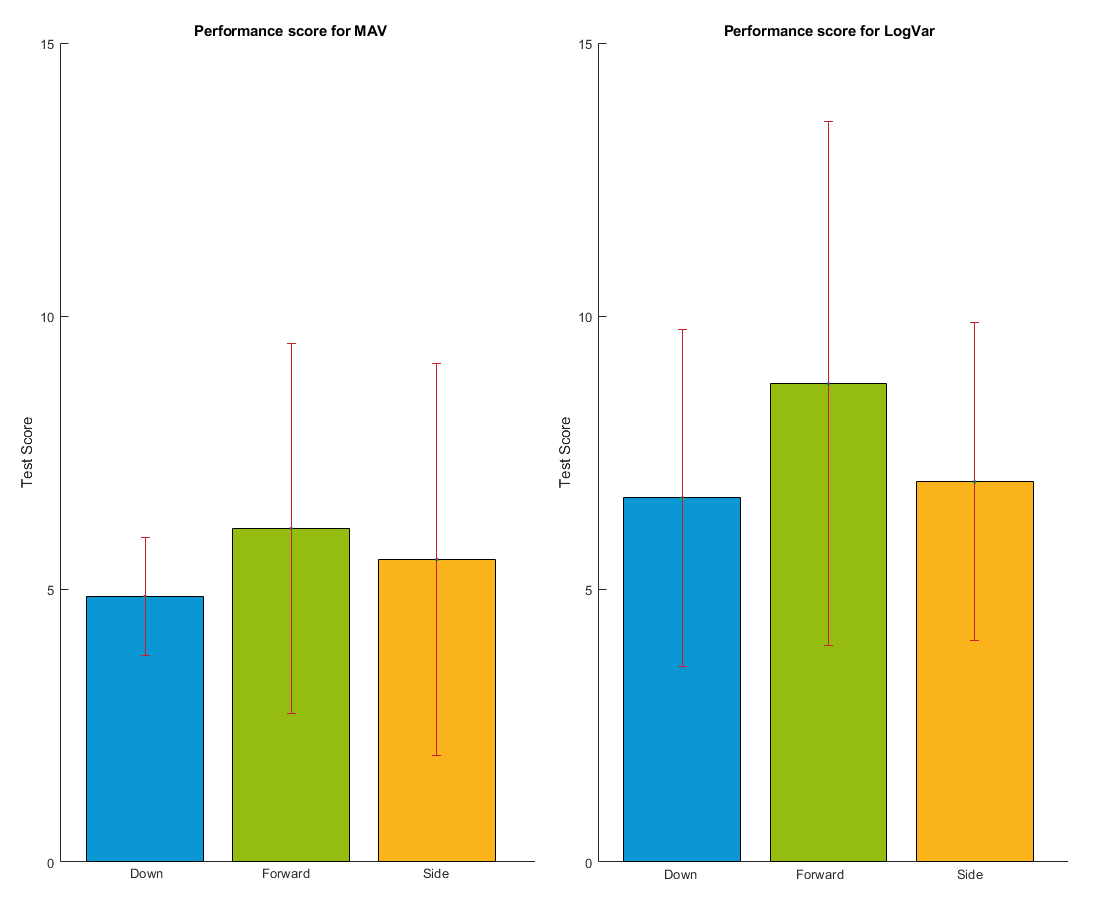
\includegraphics[width=0.7\textwidth]{figures/results/GotItTimeIMU}  %<--but is not needed.
	\caption{Calculated performance scores of the regressors with IMU data included. The bar chart illustrates the mean score across all subjects in the different limb positions, and the error bar illustrates the standard deviation}
	\label{fig:gotItTimeIMU}  %<--give the figure a label, so you can reference!
\end{figure}

	\begin{center}
		\begin{tabular}{l l l}
			\toprule
			\textbf{Limb position and feature} & \textbf{Overall mean error} & \textbf{Standard deviation}\\
			\midrule
			Down, MAV & 4.8661 & $\pm 1.0839$ \\
			Forward, MAV & 6.1094 & $\pm 3.3852$ \\
			Side, MAV & 5.5442 & $\pm 3.5847$ \\
			Down, LogVar & 6.6691 & $\pm 3.0798$ \\
			Forward, LogVar & 8.7595 & $\pm 4.7969$ \\
			Side, LogVar & 6.9652 & $\pm 2.9144$ \\
			\bottomrule
		\end{tabular}
		\captionof{table}{Test scores for the different limb for MAV and LogVar regressors with IMU included.}
	\end{center}

\begin{figure}[H]
	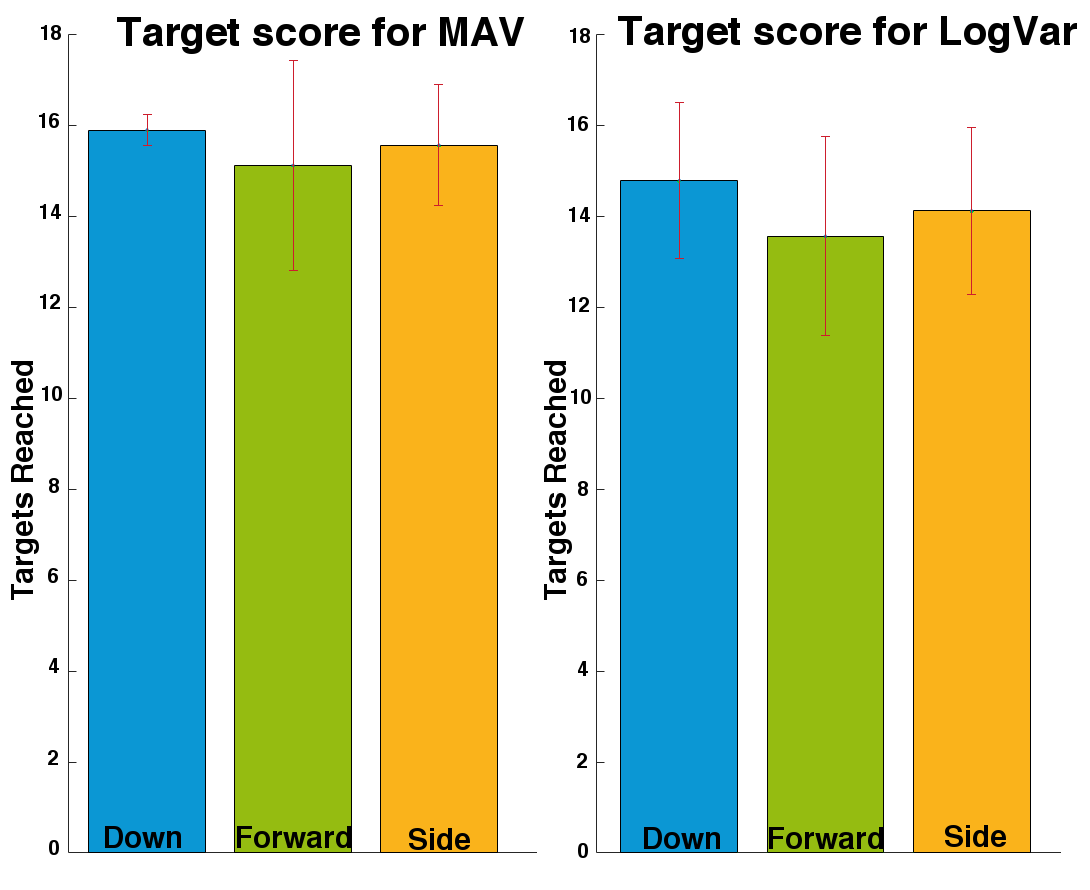
\includegraphics[width=0.7\textwidth]{figures/results/TargetsReachedIMU}  %<--but is not needed.
	\caption{The boxplot illustrates the amount of targets reached for the respective limb positions for both features with IMU data included.}
	\label{fig:TargetsReachedIMU}  %<--give the figure a label, so you can reference!
\end{figure}

	\begin{center}
		\begin{tabular}{l l l}
			\toprule
			\textbf{Limb position and feature} & \textbf{Overall mean error} & \textbf{Standard deviation}\\
			\midrule
			Down, MAV & 15.8889 & $\pm 0.3333$ \\
			Forward, MAV & 15.1111 & $\pm 2.3154$ \\
			Side, MAV & 15.5556 & $\pm 1.3333$ \\
			Down, LogVar & 14.7778 & $\pm 1.7159$ \\
			Forward, LogVar & 13.5556 & $\pm 2.1858$ \\
			Side, LogVar & 14.1111 & $\pm 1.8333$ \\
			\bottomrule
		\end{tabular}
		\captionof{table}{RMSE for the implemented LogVar regressor}
	\end{center}

\subsection{Comparison of regressors with and without IMU data}

\begin{figure}[H]
	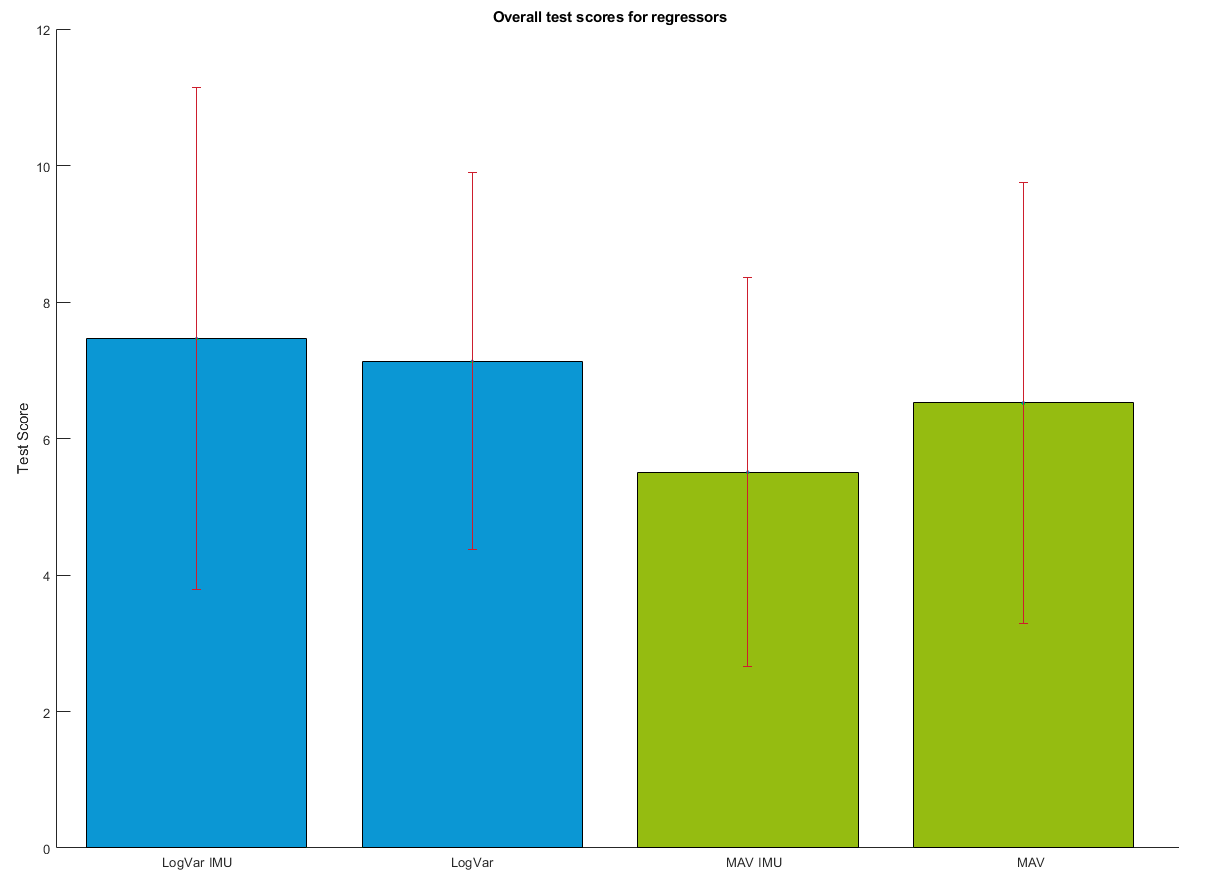
\includegraphics[width=0.7\textwidth]{figures/results/allRegressorBarzTimeScoreForTargetTest}  %<--but is not needed.
	\caption{Calculated overall performance scores of the regressors with and without IMU data included. The bar chart illustrates the mean score across all subjects, and the error bar illustrates the standard deviation}
	\label{fig:gotItTimeOverall}  %<--give the figure a label, so you can reference!
\end{figure}

\begin{center}
	\begin{tabular}{l l l}
		\toprule
		\textbf{Feature} & \textbf{Overall mean error} & \textbf{Standard deviation}\\
		\midrule
		MAV & 6.5219 & $\pm 3.2253$ \\
		MAV w. IMU & 5.5066 & $\pm 2.8477$ \\
		LogVar & 7.1284 & $\pm 2.7619$ \\
		LogVar w. IMU & 7.4646 & $\pm 3.6740$ \\
		\bottomrule
	\end{tabular}
	\captionof{table}{Average score of the target test for the four regressor designs}
\end{center}

\begin{center}
	\begin{tabular}{l l}
		\toprule
		\textbf{Feature} & \textbf{P-Value}\\
		\midrule
		LogVar w. IMU and MAV w. IMU & 0.5637 \\
		LogVar and MAV & 0.0833 \\
		LogVar w. IMU and LogVar & 0.5637 \\
		MAV w. IMU and MAV & 0.1779 \\
		\bottomrule
	\end{tabular}
	\captionof{table}{P-Values for comparison of the overall scores of the target tests}
\end{center}


\begin{figure}[H]
	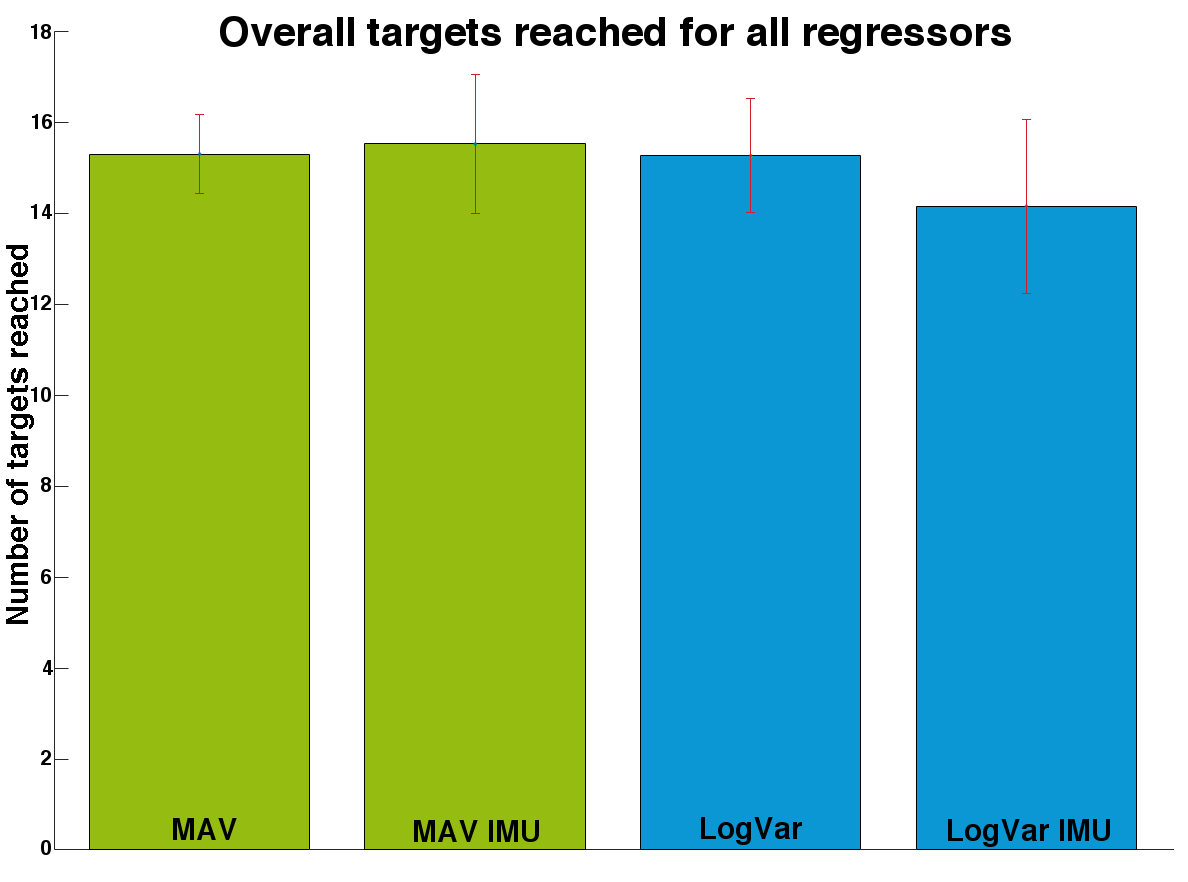
\includegraphics[width=0.7\textwidth]{figures/results/sumMoreBarsWithTargetsReachedForAllRegressors}  %<--but is not needed.
	\caption{The boxplot illustrates the amount of targets reached for all limb positions for the two features with and without IMU data included.}
	\label{fig:TargetsReachedOverall}  %<--give the figure a label, so you can reference!
\end{figure}

\begin{center}
	\begin{tabular}{l l l}
		\toprule
		\textbf{Feature} & \textbf{Overall mean error} & \textbf{Standard deviation}\\
		\midrule
		MAV & 15.2963 & $\pm 0.8689$ \\
		MAV w. IMU & 15.5185 & $\pm 1.5285$ \\
		LogVar & 15.2593 & $\pm 1.2586$ \\
		LogVar w. IMU & 14.1481 & $\pm 1.9156$ \\
		\bottomrule
	\end{tabular}
	\captionof{table}{Average number of targets reached in the target test for the four regressor designs}
\end{center}

		
\begin{center}
	\begin{tabular}{l l}
		\toprule
		\textbf{Feature} & \textbf{P-Value}\\
		\midrule
		LogVar w. IMU and MAV w. IMU & 0.0017 \\
		LogVar and MAV & 1 \\
		LogVar w. IMU and LogVar & 0.0016 \\
		MAV w. IMU and MAV & 0.0124 \\
		\bottomrule
	\end{tabular}
	\captionof{table}{P-Values for comparison targets reached in the target tests}
\end{center}